\newpage

\section{Einleitung}
Diese Planung beschreibt, wie etwas automatisch bereitgestellt wird.
Eine To-Do-App in der AWS-Cloud. Das Ziel ist es alle nötigen Komponenten automatisch 
über Infrastructure-as-Code (IaC) bereitstellen. Die Lösung besteht aus Benutzerschnittstelle, 
Backend, Datenbank und Sicherheitskomponenten.

\section{Technologieauswahl}
\subsection{Terraform als Provisionierungstool}
Als primäres Provisionierungstool wurde Terraform gewählt, da es die Plattformunabhängigkeit
ermöglicht eine Multi-Cloud Strategie und verhindert Vendor-Lock-in. 
Die deklarative Syntax in Form von HashiCorp Configuration Language (HCL) sorgt für besonders lesbare 
und wartbare Konfigurationen. Das integrierte State-Management ermöglicht eine präzise Nachverfolgung 
aller verwalteten Ressourcen. Zusätzlich profitiert das Projekt von der großen Community und der 
umfangreichen AWS-Modulbibliothek. Die Möglichkeit, wiederverwendbare Module zu erstellen, gewährleistet 
konsistente Architekturen über verschiedene Umgebungen hinweg.

Als Alternativen wurden AWS CloudFormation und Pulumi evaluiert. CloudFormation wurde aufgrund des 
potenziellen Vendor-Lock-ins ausgeschlossen, während Pulumi zwar interessante Code-basierte Ansätze 
bietet, aber die deklarative Natur von Terraform für dieses Projekt als vorteilhafter erachtet wurde.

\subsection{Architekturübersicht}
Die Architektur der To-Do-Applikation basiert auf einer modernen Serverless-Architektur in AWS. 
Im Zentrum steht ein S3-Bucket für das Frontend-Hosting, der über CloudFront als Content Delivery 
Network (CDN) bereitgestellt wird. Die REST-API-Endpunkte werden durch API Gateway bereitgestellt, 
während die Backend-Logik in Lambda-Funktionen implementiert ist. Die Datenspeicherung erfolgt in 
DynamoDB, und die Benutzerauthentifizierung wird über AWS Cognito realisiert.

\begin{figure}[h!]
\centering
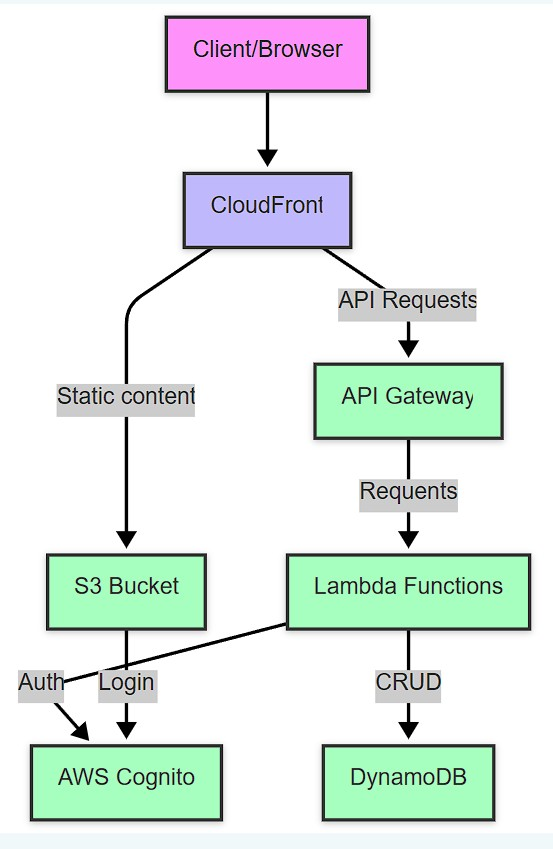
\includegraphics[width=0.8\textwidth]{fig/mermaidflowChart.jpg}
\caption{Architekturübersicht der To-Do-Applikation}
\label{fig:architektur}
\end{figure}

Die Kommunikation zwischen den Komponenten folgt einem klar definierten Fluss: CloudFront dient als 
zentraler Einstiegspunkt und leitet statische Inhalte an den S3-Bucket sowie API-Aufrufe an das 
API Gateway weiter. Das API Gateway wiederum leitet die Anfragen an die entsprechenden Lambda-Funktionen 
weiter, die für die Geschäftslogik zuständig sind. Die Lambda-Funktionen interagieren mit DynamoDB 
für CRUD-Operationen und mit Cognito für die Authentifizierung. Der S3-Bucket kommuniziert direkt 
mit Cognito für den Login-Prozess.

\section{Umsetzungskonzept}
\subsection{Authentifizierung in AWS}
Die Authentifizierung in AWS erfolgt auf mehreren Ebenen, um maximale Sicherheit zu gewährleisten. 
Für die CI/CD-Pipeline werden spezielle IAM-Rollen für Jenkins oder GitLab-Runner konfiguriert. 
Diese Rollen erhalten temporäre STS-Tokens für Ephemeral Environments, was die Sicherheit 
erheblich erhöht.

Die lokale Entwicklung wird über die AWS CLI mit benutzerbasierten Zugriffsschlüsseln ermöglicht. 
Für Produktiv-Accounts ist Multi-Faktor-Authentifizierung (MFA) obligatorisch. Sensible Daten 
werden über den AWS Secrets Manager verwaltet, der eine sichere und zentrale Verwaltung von 
Zugangsdaten ermöglicht.

Die Sicherheit wird durch strikte Anwendung des Least-Privilege-Prinzips in den IAM-Policies 
gewährleistet. Zusätzlich wird eine automatische Schlüsselrotation implementiert, um die 
Sicherheit kontinuierlich zu gewährleisten.

\subsection{Provisionierungs-Workflow}
Der Provisionierungs-Workflow ist vollständig automatisiert und beginnt mit einem Code-Commit 
im Git-Repository. Dies löst die Pipeline in Jenkins oder GitLab CI aus. Anschließend werden 
die Terraform-Konfigurationen initialisiert und ein Plan erstellt. Automatisierte Tests, 
insbesondere Security-Checks mit Checkov, stellen die Qualität und Sicherheit der Konfiguration 
sicher.

Für die Produktivumgebung ist eine manuelle Freigabe erforderlich, um ungewollte Änderungen 
zu verhindern. Nach der Freigabe wird der Terraform-Apply-Prozess ausgeführt. Der Zustand 
der Infrastruktur wird in einem S3-Bucket mit Locking-Mechanismus gespeichert, um 
Konflikte bei parallelen Änderungen zu vermeiden.

\section{Vor-/Herausforderungens}
\subsection{Vorteile}
Die gewählte Architektur bietet zahlreiche Vorteile. Durch die Verwendung von Infrastructure-as-Code 
werden identische Umgebungen gewährleistet, was die Konsistenz über verschiedene Deployment-Stages 
hinweg sicherstellt. Die vollständige Provisionierung kann in weniger als 10 Minuten abgeschlossen 
werden, was die Geschwindigkeit der Entwicklung und des Deployments erheblich steigert. Die 
Kostentransparenz wird durch konsequentes Tagging aller Ressourcen gewährleistet. Die Sicherheit 
profitiert von der versionierten Konfiguration, die Compliance-Anforderungen erfüllt.

\subsection{Herausforderungen}
Trotz der vielen Vorteile gibt es auch Herausforderungen zu bewältigen. Die Terraform-Syntax und 
die AWS-Services erfordern eine gewisse Einarbeitungszeit. Das Zustandsmanagement erfordert ein 
sorgfältiges Handling der state-Dateien, um Konflikte zu vermeiden. Die Fehlersuche bei 
Abhängigkeitsproblemen kann komplex sein und erfordert ein tiefes Verständnis der 
Infrastruktur-Komponenten.

\section{Technische Umsetzung}
\subsection{Terraform-Modulstruktur}
Die Terraform-Konfiguration ist in logische Module aufgeteilt, die jeweils spezifische 
Aspekte der Infrastruktur verwalten. Die Module umfassen Netzwerk, Datenbank, Backend, 
Frontend und Sicherheit. Diese Struktur ermöglicht eine klare Trennung der Zuständigkeiten 
und erleichtert die Wartung und Erweiterung der Infrastruktur.

\subsection{Beispiel: DynamoDB-Provisionierung}
Ein konkretes Beispiel für die Provisionierung ist die DynamoDB-Tabelle für die To-Do-Items. 
Die Tabelle wird mit Pay-per-Request-Billing konfiguriert, was eine kosteneffiziente 
Skalierung ermöglicht. Die ID wird als Hash-Key definiert, und die Tabelle wird mit 
entsprechenden Tags für die Umgebung und das Management versehen.

Die automatisierte Provisionierung mit Terraform ermöglicht reproduzierbare, sichere und 
kosteneffiziente AWS-Umgebungen für die To-Do-Applikation. Durch modularen Code und 
CI/CD-Integration wird der Entwicklungslebenszyklus optimiert.